\subsection{Die Natürlichen Zahlen}
Symbol: $\mathbb{N}$\\
sind alle Ganzen Positiv Zahlen

\hfill \break
\hfill \break
$ \mathbb{N}=\{0,1,2,3,4,5,6,\ldots\} $

\hfill \break
$ \mathbb{N}^{*}=\{0,1,2,3,4,5,6,\ldots\} $

\hfill \break
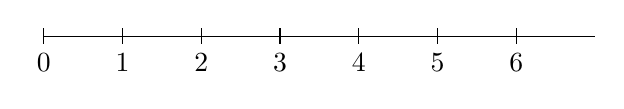
\begin{tikzpicture}
    \draw (0,0) -- (7,0);
    \foreach \X in {0,...,6}
    \draw (\X,0.1) -- (\X,-0.1);
    \foreach \X in {0,1,2,3,4,5,6}
    \node[anchor=north] at (\X,-0.1){\X};
\end{tikzpicture}

\hfill \break
Möglichkeiten mit den Natürlichen Zahlen:
\begin{enumerate}
    \item Addieren ist uneingeschränkt möglich:
          \begin{itemize}
              \item 1+3 = 4
              \item 10+5 = 15
          \end{itemize}
    \item Subtrahieren ist nur eingeschränkt möglich:
          \begin{itemize}
              \item 1-3 = ?
              \item 10-5 = 5
          \end{itemize}
    \item Multiplizieren ist uneingeschränkt möglich:
          \begin{itemize}
              \item 1*3 = 3
              \item 10*5 = 50
          \end{itemize}
    \item Dividieren ist nur eingeschränkt möglich:
          \begin{itemize}
              \item 1/3 = ?
              \item 10/5 = 2
          \end{itemize}
\end{enumerate}